\chapter{Introduction}
With the ongoing digital transformation it seems only a matter of time until the shift from paper based ballots to electronic voting (e-voting). Recent polls show that the majority of the Swiss population is interested in having the possibility to vote online \footnote{\url{https://www.swissinfo.ch/ger/umfrage_grosse-zustimmung-zu-e-voting-trotz-sicherheitsbedenken/42457426}}. However, e-voting is a very complex topic and designing a secure e-voting protocol is notoriously challenging in terms of IT-security and cryptography.

\section{Electronic Voting}
First trials with e-voting in Switzerland date back to 2003 \cite{swissinfo}. Since 2015, it has been possible for Swiss citizens registered in the cantons of Geneva and Neuchâtel and living abroad to vote electronically \cite{aso}. These systems were available only for a limited electorate size since they did not yet meet the requirements in terms of security and transparency to be accepted as a secure e-voting platform on a nationwide scale.

An e-voting system must satisfy a large variety of security requirements set up by the government, including:

\begin{itemize}
 \item Privacy: no one can find out information about a voter's candidate selection. This implies that a voter's ballot must be encrypted before it leaves the voter's client and until the election is tallied.
	\item Fairness: no one is able to learn the intermediate result or the outcome of an election before the result has been officially tallied and published to a public board.	
	\item Authenticity: all voters must be authenticated as eligible voters in order to cast a vote.
	\item Soundness: only valid votes are being tallied. If a voter selects more candidates than he is allowed to or less than he is supposed to, the vote must not be counted.
	\item Robustness: an e-voting system detects cheating actors.
	\item Distribution of Trust: the security of an e-voting system must not rely on a single point of trust.
\end{itemize} \cite{evotinganforderungen}

There exist many different concepts and e-voting protocols that cover many of the basic requirements. However, existing solutions typically behave like a black-box and keep the internals hidden, such that a voter cannot be sure whether his vote has been recorded correctly and counted in the final result.

A common problem is the \textbf{insecure platform problem}: if a voter's computer is affected by malware, the vote casting process is no longer under the voter's control and the candidate selection could be possibly manipulated without the voter's notice. It must be \textbf{individually verifiable} to every voter that his intended vote has been recorded, while at the same time the voter's privacy must still be ensured at all times \cite{chvote}.

One of the requirements that is the hardest to achieve is the \textbf{universal verification}: a good e-voting system must be transparent and allow an external person to verify that every protocol participant has abided by the protocol and that all and only valid votes have been counted correctly.

Should an e-voting system be available to more than 30\% of the respective cantonal electorate, it must be individually verifiable; if 50\% - both individually as well as universally \cite{evotinganforderungen}.

\section{CHVote Protocol}
Some of the mentioned requirements might sound as a paradox at first. However, they can be solved by advanced cryptography. A contract was formed between the state of Geneva and the  Research Institute for Security in the Information Society (RISIS) of the Bern University of Applied Sciences to work out a new protocol which meets the complex requirements set up by the Swiss government. In 2017, Rolf Haenni, Reto E. Koenig, Philipp Locher and Eric Dubuis published the resulting specification document and a proof-of-concept has been successfully implemented by the State of Geneva. Geneva is currently developing a new version of their e-voting system with the name CHVote, based on these specifications. Other cantons, currently St. Gallen, Aargau, Bern and Lucerne have announced their interest in cooperating with Geneva and might use their system in future.

The CHVote specifications document is publicly available and describes not only the theoretical background but also provides pseudocode for the approximately 60 algorithms that are needed to implement their protocol.

Chapter 3 will summarize the most important aspects of the CHVote specifications for a better understanding of our work.

\section{Project Task}
An additional problem with which e-voting is confronted is that understanding such a complex protocol is not easy without good knowledge of cryptography and mathematics. This might be one of the reasons why many people still do not trust electronic voting systems.

In close consultation with the authors of the CHVote specifications, we were looking for an interesting project for our bachelor thesis in the thematic field of e-voting. We decided to study the CHVote specifications, implement the protocol and build an application on top of it.

\begin{center}
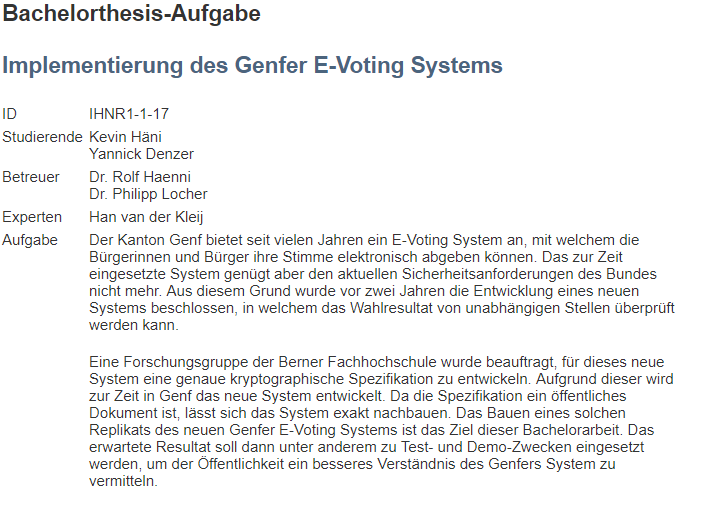
\includegraphics[scale=0.95]{assets/aufgabe.png}
\captionof{figure}{The initial task description of the bachelor thesis left a number of open possibilities as to how exactly the project could be implemented. Specific tasks and requirements were discussed with our supervisors during the first few weeks of the project.}\label{Bachelor thesis task}%
\end{center}

Based on the initial, rather general task description (see figure \ref{Bachelor thesis task}), there were several possibilities regarding the final product, such as a realistic prototype, a verifier software for the implementation which is being developed in Geneva, or an application that targets the educational problem and can be used to demonstrate the functionality of the new protocol.

Ultimately, we have decided to implement the last option: the goal of our project was to develop a web-based application which allows to visualize every step of a CHVote election event, from the pre-election tasks like generating the electorate data, casting and confirming ballots from a voter's point of view, to the post-election processes like mixing, decryption and tallying. The main goal of our project was not to implement a secure, "ready for production" e-voting system from an infrastructural perspective, but more the visualization and the user-interface. With the resulting application users would be allowed to get a hands-on experience with Geneva's new e-voting system and a preview of how the future of voting in Switzerland might possibly look like.

Studying of the specifications and the development of the approximately 60 algorithms that were defined as pseudocode in the specifications was done as preparatory work during the course "{}Project 2"{}, which we had finished just before the start of the bachelor thesis. The resulting set of algorithms have been used as a library for implementing the protocol on which our application is built.

Outline of this document: in chapter 2 we will further discuss the goals and requirements that we have set for this project. Additionally, it covers the time planning and the project methodology.

For better understanding of our application, chapter 3 contains a short summary of the CHVote specifications document and establishes the terminology and theoretical background.

Chapter 4 will describe the final product and the concepts behind our application.

Chapter 5 covers the technical aspects regarding the implementation, such as the architecture, the language and technology decisions. Later sections contain detailed information about the internals of each component of our application and the challenges we were facing during the implementation phase.

Chapter 6 will conclude this document with a short summary and a reflection about the project.
